\chapter{Conclusion}\label{ch:Conclusion}

In this Chapter a summary of the work presented in this thesis is provided, with the work evaluated against the research aims outlined in Chapter \ref{ch:intro}. Next, potential avenues for future research are explored. 

\section{Thesis Summary}\label{ch:Conclusion,sec:Summary}

Motivated by the problem space as outlined in Chapter \ref{ch:intro}, this thesis explores the use of computer vision and deep learning for the task of automated photo-id catalogue curation and most likely matching. Before beginning work to fulfil the thesis' aims, Chapter \ref{ch:Background} provides the relevant background knowledge required for understanding work described in later Chapters; this includes an introduction to current photo-id methodology, deep learning and computer vision fundamentals, and the current state-of-the-art in photo-id aides. It is here where the problems with current approaches are evaluated in detail, providing further justification for the work undertaken in this thesis. 

In Chapter \ref{ch:cetDet} the first step towards automatic photo-id catalogue management is tackled through the development of a coarse-grain detector capable of generating mask predictions for above water fieldwork imagery, focussing on dolphins as the cetacean species of interest. The environmental and technical requirements of the detector are outlined for use as success metrics, whilst the use of mask predictions rather than bounding boxes is justified. To this end, a Mask R-CNN \cite{he_mask_2017} detector is developed, trained using data  containing examples of Indo-Pacific bottlenose dolphins collected by Newcastle University's Marine MEGAfauna Lab whilst on expedition to Zanzibar, Tanzania in 2015 \cite{sharpe_indian_2019}. 

During model development the use of transfer learning and various data augmentation strategies are explored, helping to mitigate the issues inherent with training deep computer vision models using dataset sizes typical of photo-id surveys. Model hyperparameter optimisation is then performed, before the best performing model on the Zanzibar data is determined. This optimal model achieves high mean average precision (mAP) over a range of key intersection over union (IOU) thresholds, confirming coarse-grain detection of cetaceans is possible even in noisy environments and where large variation in the region of interest is present. 

This best model is then utilised to explore the post-processing techniques required to allow for a reduction in the computational expense of downstream models and the removal of unneeded background noise, whilst at the same time ensuring no useful individually identifying markings are lost. The ability to achieve this highlights that it is possible to fully remove the need for the data pre-processing which is currently performed by cetacean researchers, either when performing photo-id matching manually or with the use of aides.

In Chapter \ref{ch:NDD} the developed detector's robustness to species of interest and spatio-temporal changes are evaluated. To achieve this, fieldwork was undertaken alongside Newcastle University's Marine MEGAfauna Lab to create a photo-id catalogue of resident bottlenose and white-beaked dolphins present in the waters around Northumberland, UK, during Summer 2019. Once complete the photo-id catalogue was converted into a dataset useful for computer vision model training, called the Northumberland Dolphin Dataset 2020 (NDD20). Using this data, it can be seen that the detector is capable of high mAP at a range of IOU thresholds, confirming the model is robust to species of interest and spatio-temporal changes. As such, this suggests that no model fine-tuning or re-training is required for use in future photo-id surveys provided the model is trained to a high accuracy using previously obtained imagery. 

Detections from NDD20 are then post-processed to produce a second dataset representative of detector output, allowing for the training of the next model in the pipeline. Additional imagery of the individuals provided by the University of Aberdeen and the University of St Andrews are also included in the identification training dataset, called NDD AU SMRU, as a 23 individual overlap was determined between the catalogue created for Northumberland and those for Eastern Scotland held by the partner institutions. This additional data helps combat the issue of small dataset size when performing model training. 

In Chapter \ref{ch:ID} a model capable of fine-grain, few-shot cetacean re-identification is created, aiding researchers by vastly reducing their search space when performing catalogue matching. Beginning by outlining the requirements this model must adhere to, two possible approaches are evaluated. Through this, the use of a Siamese Neural Network (SNN) based approach is determined most suitable. Model training is performed using two distinct backbone architectures; a relatively simple one called EmbeddingNet and a more complex one known as VarvaraNet based on work by Vetrova \textit{et al.} \cite{vetrova_hidden_2018}. The use of pairwise or triplet ranking losses is explored, as well as online semi-hard triplet mining and hyperparameter tuning via Bayesian optimisation. A range of models were generated, trained using the previously created NDD AU SMRU dataset. Evaluation of the models was performed using top-1, top-5, and top-10 accuracies. The best performing model, a VaravarNet trained without the use of any data augmentation, is capable of vastly reducing the search required by a cetacean researcher when performing most likely catalogue matching. 

The ability of SNNs to allow for the flagging of potentially previously uncatalogued individuals is also explored. Thanks to the model's capability to reduce a high dimensional input down to a low dimensional representation, or embedding, existing catalogue examples can be plotted into a latent space such that they create class clusters. By utilising class prototypes and Euclidean distance measurements, as well as the K-Nearest Neighbours algorithm, this Chapter shows that the flagging of potentially previously unseen individuals can be achieved. Any new individuals which are added to the catalogue can also easily be added to the model without the need for re-training thanks to embedding clustering and class prototyping. Further experimentation using a modified version of NDD AU SMRU presents some evidence to suggest that splitting individual classes in two based on which side of the dorsal fin is captured may lead to improved model performance, but further tests are required to confirm this. 

In Chapter \ref{ch:SNNEvaluation} the robustness of SNNs for the task of most likely catalogue matching is explored. The effects of dataset variation on model performance are quantified, with experimentation suggesting that the retention of background noise through the use of bounding box detections leads to inflated model performance when data has been collected over a small temporal scale. This presents evidence to suggest that the initial decision to perform full background removal through the use of masks was the correct decision, even at the expense of greater computation, and may present an inherent flaw in other photo-id aides which do not remove all background. 

The generalisability of catalogue matching using SNNs is further evaluated through the use of a second photo-id catalogue, provided by the Sarasota Dolphin Research Program. Work here shows that whilst catalogue matching can be performed on other datasets, rather than there being something inherent to the NDD AU SMRU dataset which made this possible, a photo-id catalogue must first exist in order for training to take place. Further, the threshold values utilised in uncatalogued individual thresholding must be tuned. Finally in Chapter \ref{ch:Conclusion}, the work undertaken in this thesis is summarised, its contributions outlined, and avenues for future research explored. 

\section{Evaluation Against Thesis Aims}\label{ch:Conclusion,sec:AimsEvaluation}

As outlined in Chapter \ref{ch:intro}, the aim of this thesis was to \textbf{design, implement, and evaluate a system for fully automatic catalogue matching based on unprocessed photo-id fieldwork imagery}. This was then separated into four research questions (detailed in Section \ref{ch:intro,sec:AimsAndContributions}), each of which should be answered in an attempt to fulfil the overall research aim. 

The first question asks whether it is possible to remove or greatly reduce the need for manual pre-processing of photo-id data in a fully automated way through the use of coarse-grain detection. Work undertaken in Chapter \ref{ch:cetDet} answers this question, proving that it is indeed possible. The model developed during this Chapter is capable of producing highly accurate detections when evaluated using a variety of mAP@IOU thresholds. Through training on unprocessed fieldwork data, the model is able to detect highly variant regions of interest in large-scale, noisy, above water photo-id imagery. When coupled with the developed detection post-processing methodology, the need for manual data pre-processing, such as cropping or rotation, is removed. If pre-processing of photo-id data was required for means other than most likely catalogue matching, or researchers did not wish to pass the data downstream, then the model could be used as a stand-alone system for quickly cropping down fieldwork imagery to only the dorsal fin. 

The second question posits if it is possible to perform detection post-processing in such a way as to both reject likely false positives and remove noise whilst retaining identifiable markings present on the animals. The post-processing methodology outlined in Chapter \ref{ch:cetDet} confirms this is possible. The use of a \textit{dolphin-like} colour threshold, described in Section \ref{ch:cetDet,sec:postProcessing,sub:colourThresholdingMaskComponents} allows for the removal of likely erroneous detections whilst keeping those which are over-exposed but correct, reducing the false-positive retention rate. Further, the inclusion of morphological transformations ensures that any identifying information on the dorsal fin which may have been missed is included in the detection, provided the information is surrounded by pixels which have been correctly classified. Coupled with background removal and cropping, this ensures unneeded noise is removed whilst identifiable markings are retained. 

The third question asks if it is possible to perform highly accurate most likely photo-id catalogue matching based on extreme fine-grain information, even when operating on few-shot data. Work undertaken in Chapter \ref{ch:ID} confirms this can be achieved through the use of an SNN trained using online semi-hard triplet mining. The model is capable of producing sufficiently distinct embeddings for classes within the extreme fine-grain NDD AU SMRU dataset, where there is small inter-class but high intra-class variation. Further, the dataset is also few-shot given the free roaming nature of the individual animals present. 

High top-1, top-5, and top-10 accuracies are achieved on this dataset, confirming highly accurate automated most likely photo-id catalogue matching is possible. This is further confirmed through evaluation of the approach against the SDRP dataset, where high accuracies are once again obtained. 

Finally, the fourth question asks how generalisable the models created throughout this work are to changes in species of interest and spatio-temporal shifts. In Chapter \ref{ch:cetDet}, the coarse-grain cetacean detector is shown to be highly robust to these changes. High mAP is observed at a range of IOU thresholds on previously unseen photo-id catalogue data collected in a different spatio-temporal area, and containing two new cetacean species, than on that which the model was trained. The approach to most likely catalogue matching is also shown to be generalisable, achieving high accuracies on both the NDD AU SMRU and SDRP datasets in Chapters \ref{ch:ID} and \ref{ch:SNNEvaluation} respectively. However, greater limitations on the generalisability of the catalogue matching model are observed when compared to the dorsal fin detector, as this model requires retraining on the new photo-id catalogue and new thresholds for potentially uncatalogued individual thresholding must be located. 

In summary, as all research questions have been answered it can be stated that the work undertaken in this thesis has achieved its aims. 

\section{Future Research Directions}\label{ch:Conclusion,sec:FutureWork}

This Section describes several interesting topics for future research which builds upon work undertaken in this thesis.

\subsection{Effect of Initial Catalogue Size on Most Likely Matching}\label{ch:Conclusion,sec:FutureWork,sub:EffectOfCatalogueSize}

Performance of a model for the task of most likely matching has been shown to be influenced by initial catalogue size, most notably in Sections \ref{ch:SNNEvaluation,sec:EffectOfAUSMRU} and \ref{ch:SNNEvaluation,sec:SDRP,sub:SDRPDataset,sub:reversedSDRP}. Due to the data-hungry nature of training deep computer vision models, and the relatively small amounts of data available to this work, it was not feasible to explore in detail the effect of initial catalogue size on model performance. Work by Wu \textit{et al.} \cite{wu_sampling_2017} has shown that training data can impact embedding generation as much as the chosen loss function. As such, it is highly likely that embedding generation is improved the more training data is provided, allowing the model to create better defined class clusters. This will in turn allow for improved detection of potentially uncatalogued individuals. 

Due to the lack of data availability in this space, caused by an apprehension for cetacean researchers to release all data they have on resident populations (thanks to issues ranging from conservation of the animals and their habitat to safeguarding their own lab's future research), it was not possible to obtain a large scale, multi-year catalogue. Initials plans for this work included the provision for data collection around the Northumberland coastline with the goal of increasing the data available in the Northumberland Dolphin Dataset. These plans were scuppered due to the unforeseen health situation from 2020 onwards which prevented fieldwork surveys from occurring. 

This lack of data availability meant that a meaningful study into the effect of initial catalogue size on most likely matching performance was not possible. A study like this is extremely important, as it would provide researchers with some minimum number of images they would need in order to make use of a system like the one presented in this work. As such, future research should endeavour to ensure that a study like the one described is undertaken. Understanding the relationship between embedding generation and catalogue size may also allow for the development of a metric alerting researchers to data drift (discussed in more detail in Section \ref{ch:ID,sec:ModelSelection,sub:limitations}).

\subsection{Effect of Background Over Large Temporal Scales}\label{ch:Conclusion,sec:FutureWork,sub:EffectOfBackgroundOnLargeTemporalScales}

The provision of a large multi-year catalogue would also allow for a study into the effect of background noise over large temporal scales. Work undertaken in Section \ref{ch:SNNEvaluation,sec:EffectOfNoise} suggests that, when utilising bounding box detections instead of pixel-wise masks, embedding generation is influenced more by the retained background than the region of interest (RoI), provided the background is feature heavy. This is hypothesised to be caused by the small temporal scale over which the images were collected; the background remains mostly consistent even though the RoI changes greatly due to the fast roaming nature of the animals. 

If a dataset could be obtained which consisted of a large number class examples with wide variation in the background, a property inherent of a multi-year dataset due to its broad temporal scale, then the effect of background on embedding generation could be fully quantified. At present, it is unclear if embeddings will always be influenced regardless of background variation or if the model will learn to generate embeddings which ignore this. If it is the former, then this has wide ranging implications for the development of future photo-id aides, and may provide reason to further examine the performance of current aides which perform matching without full background removal such as finFindR \cite{thompson_finfindr_2022} or Lee \textit{et al.} \cite{lee_backbone_2020}. 

Exploration into the use of domain generalisation techniques should also be explored to reduce the effect of background on embedding generation. Recent years have seen the publication of a wide range of generalisation techniques for image representation \cite{zheng_exploiting_2019, yan_clusterfit_2020, creager_environment_2021, zhou_domain_2022, tommasi_domain_2015, cohn_improving_1994, neyshabur_exploring_2017}, and it may be the case that the use of one or more of these may help the SNN focus on features present in the RoI rather than the background. Further, the use of out of distribution training data may prove beneficial. Work undertaken by Lee \textit{et al.} \cite{lee_weakly_2022} showed that computer vision models may confuse background cues to be a foreground concept due to correlation, for example thinking railway tracks are part of trains as they are always shown together in training images. By providing explicit negative example (e.g. images containing tracks only), the model is able to shift its understanding of what constitutes a train. Advances in the domain of person re-identification may also be applicable here, helping to reduce the bias introduced through background inclusion \cite{nguyen_background_2016, huang_sbsgan_2019, tian_eliminating_2018}. Utilising these techniques during model training may make it possible to shift embedding generation focus away from the background. 

\subsection{Further Per-Side Experimentation}\label{ch:Conclusion,sec:FutureWork,sub:MorePerSide}

Section \ref{ch:ID,sec:perSide} outlines experimentation performed using the NDD AU SMRU dataset to examine whether automated photo-id matching should, like its manual counterpart, split individual classes on a per-side basis. Results obtained suggest that training an SNN on a per-side basis improves model performance, reduces embedding dimensionality, and necessitates a less computationally expensive backbone architecture.

It was not possible to recreate this experiment however using the SDRP dataset due to the limited number of examples per class. As such it cannot be said with certainty whether splitting classes based on the side of the dorsal fin visible is optimal regardless of the data, or if there is a property inherent to the NDD AU SMRU dataset that results in increased model performance and reduced complexity when split which is not observed in photo-id catalogues globally. If more data was obtained to facilitate aforementioned future research, the generalisability of a per-side approach could also be validated.  

\subsection{Creating a Generalised Model for Catalogue Matching}\label{ch:Conclusion,sec:FutureWork,sub:GeneralSNN}

One limitation of the model utilised for most likely matching currently is the need to re-train the SNN for each photo-id catalogue. As a result, initial manual curation must be performed before the methodology can be applied. The threshold values required for uncatalogued individual detection through both Euclidean distance measurement between class prototypes and the K-Nearest Neighbours algorithm are also shown to be dataset dependant thanks to work outlined in Sections \ref{ch:ID,sec:ModelSelection,subsec:UncataloguedIndividualThresholding} and \ref{ch:SNNEvaluation,sec:SDRP,sub:uncatalogued}. It may be the case that determining these threshold values can be automated by utilising the properties of the latent space and the training data embeddings, an approach which should be explored in future.

The feasibility of a more general SNN capable of catalogue-agnostic photo-id should be examined in future research. There is little published work examining the feasibility of generalised SNNs however, with only work by Melekhov \textit{et al.} \cite{melekhov_siamese_2016} suggesting it is possible to create a generalised SNN for the task of landmark recognition. It may be the case that training a catalogue-agnostic model is not possible due to the extreme fine-grain nature of the classes, but future research should confirm this. 

It should be noted however that these limitations do not apply to the detector model, which has been found in Section \ref{ch:NDD,sec:EvalUsingNDD20,subsec:geographyTimeSpeciesChange} to not require re-training when applied to new photo-id catalogues.

\subsection{Expansion to Other Data Subjects}\label{ch:Conclusion,sec:FutureWork,sub:Underwater,Video,OtherCetaceans}

Work undertaken in this thesis has focussed on photo-id imagery of dolphins captured from above the waterline. Future work should endeavour to expand the developed pipeline for use with other cetacean species, such as whales and porpoises, other marine life, and terrestrial species. Furthermore, the use of below water photo-id imagery \cite{van_bressem_visual_2018} and video data should be explored. It is expected that a change in data subject would necessitate re-training of both the coarse-grain detector and the fine-grain catalogue matcher models although similarly high levels of performance as presented throughout this thesis are considered likely provided sufficient amounts of data are utilised. 

\subsection{Transforming the Model Pipeline}\label{ch:Conclusion,sec:FutureWork,sub:Transformers}

In 2017 the domain of Natural Language Processing (NLP) was revolutionised thanks to the introduction of the Transformer model architecture, introduced by Vaswani \textit{et al.} \cite{vaswani_attention_2017}. Up until this point, tasks like sentiment analysis or text translation were dominated by models based around long short-term memory \cite{hochreiter_long_1997} or recurrent neural networks \cite{rumelhart_learning_1985}. 

The Transformer architecture makes use of attention, a mechanism which allows a model to understand long-range interactions between values in a sequence. This removes the need for recurrence, allowing for the parallelisation of training. As a result, the state-of-the-art for a range of NLP tasks is now dominated by Transformers \cite{brown_language_2020, devlin_bert_2019, ng_facebook_2019, wolf_transformers_2020}. 

It wasn't until 2021 however that Transformers entered the vision space, thanks to work by Dosovitskiy \textit{et al.} \cite{dosovitskiy_image_2021}. By splitting images into fixed size patches, analogous to words in a sentence as seen in Figure \ref{fig:vit}, the authors show that it is possible to remove the need for convolution (the basis of convolutional neural networks (CNNs), see \ref{ch:Background,sec:CNN,sub:CNN}) and utilise attention for the task of image classification. 

\begin{figure}[h]
	\begin{center}
		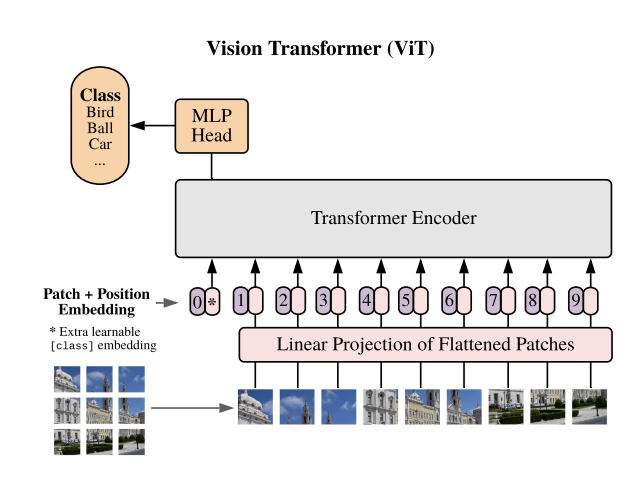
\includegraphics[scale=0.7]{Chapter7/figs/vit.png}
	\end{center}
	\caption{Example Vision Transformer architecture. Image from \cite{dosovitskiy_image_2021}.}
	\label{fig:vit}
\end{figure}

Since then Vision Transformers (ViTs) have been utilised for a variety of computer vision tasks such as object detection \cite{fang_you_2021, li_exploring_2022}, segmentation \cite{hu_istr_2021, prangemeier_attention-based_2020, wang_end--end_2021}, and image similarity \cite{el-nouby_training_2021}, often achieving state-of-the-art performance on large scale benchmark datasets. Future work should focus on examining potential performance improvements through conversion of the coarse-grain detector and fine-grain catalogue matcher models to ViTs. It should be noted here however that this is very much a long term goal as Transformers currently require both massive amounts of data and time to train - with the original ViT models trained on the JFT-300M dataset \cite{sun_revisiting_2017}, containing 300 million images, for up to 12.3k TPUv3-core-days. As such, it is not currently possible to train a ViT for the work undertaken in this thesis, but this does not mean it will not be possible in the future through improvements in architecture or training schedule, or via fine-tuning. Further, the use of hybrid approaches should also be explored, which make use of elements from both ViTs and CNNs \cite{liu_convnet_2022, liu_swin_2021}.

\subsection{The Creation of a Working Computer Program}\label{ch:Conclusion,sec:FutureWork,sub:GUI}

Figure \ref{fig:pipeline}, shown at the beginning of this document, highlights the expected data flow between the proposed components. Throughout the course of this thesis, these components are created and it is shown how they can be connected together to form a fully automated photo-id curation system. However, the work undertaken stops short of actually implementing these connections and creating a working computer program which can be utilised by cetacean researchers. 

\newpage

As such, future work should focus heavily on program development. This would include not just MLOps and data engineering work to connect the pipeline's components together \cite{zhou_towards_2020}, but also the development of a backend database for the storage of photo-id imagery embeddings, and a frontend graphical user interface (GUI) to facilitate researcher interaction with the pipeline in a familiar and friendly way - work considered beyond the scope of this thesis. Once created however, a working computer program would allow for an in-depth study into the time savings provided by an automated photo-id aide such as the one presented here compared to performing catalogue matching manually, as well as allow cetacean researchers globally to make full use of the techniques outlined in this thesis. 

